\externaldocument{Developerdocumentation}
\chapter{Architecture Overview}
This chapter gives a brief overview of the architecture.

\section{Overview over the Architecture}

\begin{figure}[htbp] 
  \centering
  \begin{minipage}[b]{1\textwidth} 
    \caption{Overview-Architecture of KernelHaven}\label{fig:arch_simple}
    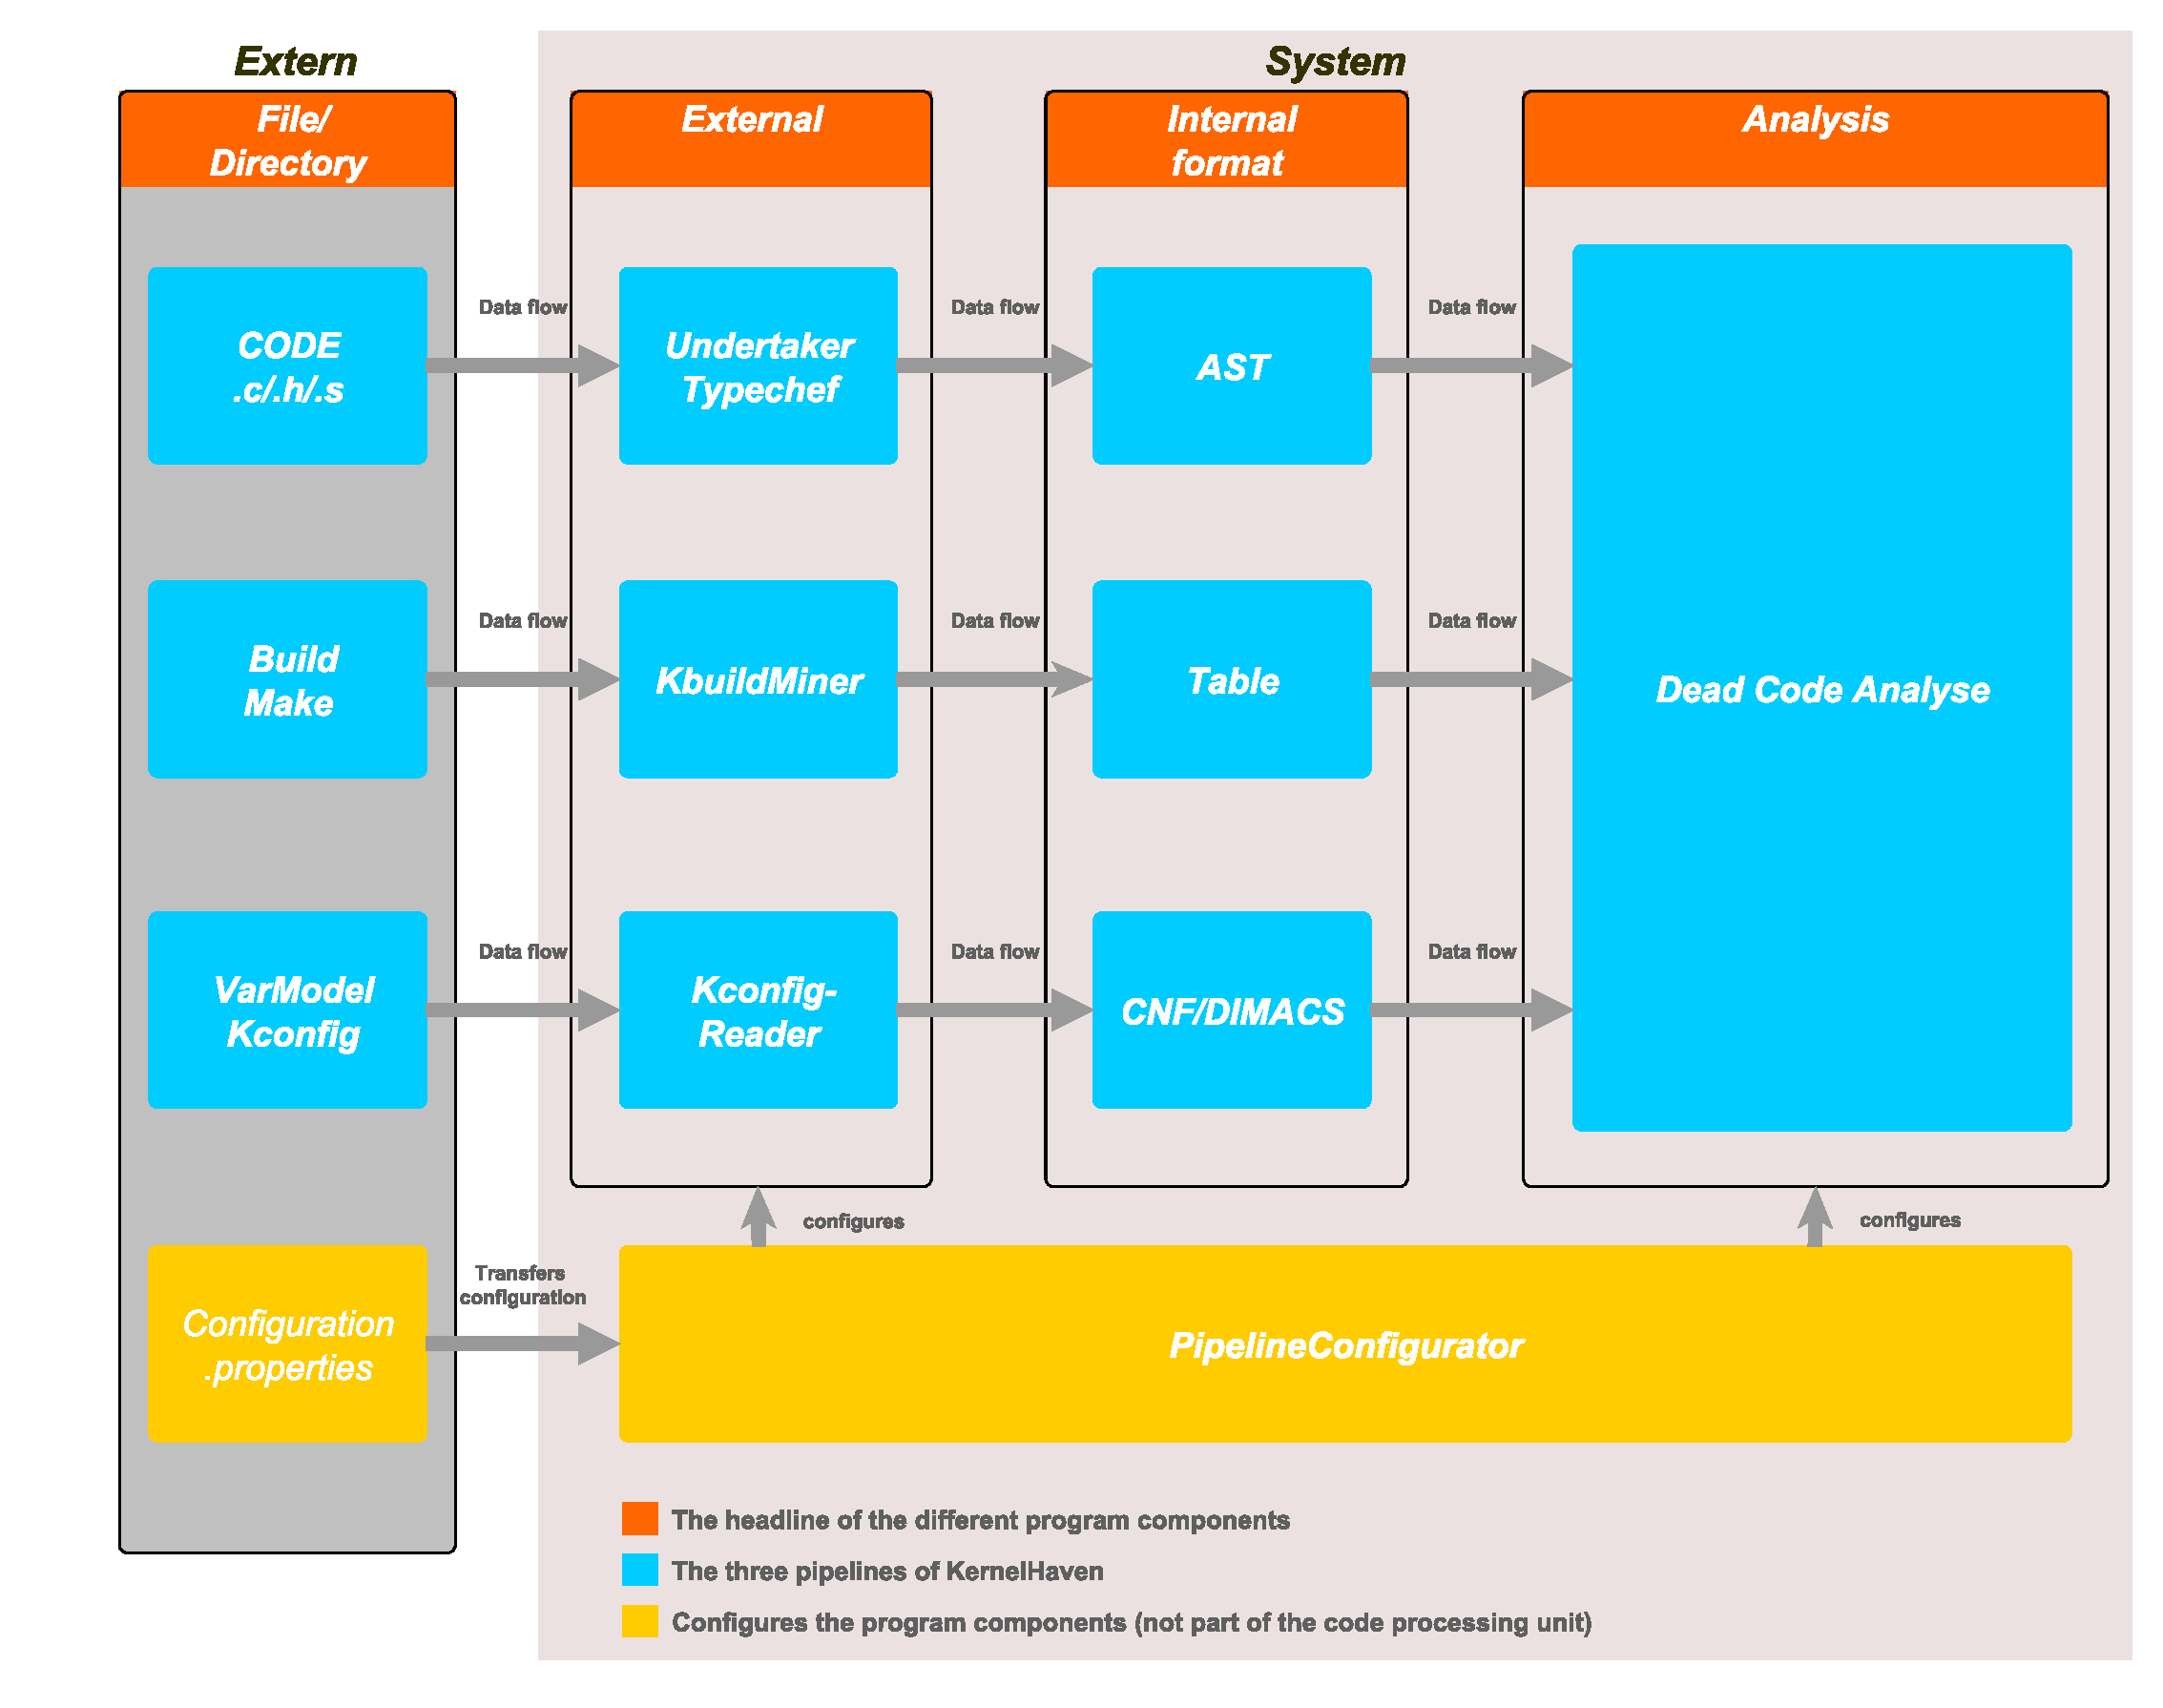
\includegraphics[width=1\textwidth]{Bilder/arch_simple.pdf}
  \end{minipage}
\end{figure}

\smallskip
In \autoref{fig:arch_simple} is an overview of the KernelHaven architecture, detailed information about how the execution works and about every component of the architecture are described below.

An execution works as follows:

After the pipeline is set up (see pipeline configuration below) , the analysis component starts the providers, which in its turn starts the extractors. Each extractor spawns a separate thread, so that the three pipelines and the analysis can run in parallel. When an extractor is finished, it tells its provider about the result. When the analysis queries the result, the provider waits until the result is present and returns it to the analysis. This way, the providers function as a mediator between the analysis and the extractor threads.

If an extractor encounters an exception, it passes an extractor exception to the provider. After that, each call from the analysis to the get function of the provider will throw this exception. This way the analysis is properly notified about exceptions.

If caching is enabled in the configuration, then the providers will first try to read the result from the cache. In this case, the extractors are only started if the cache does not contain the required data.

The pipeline is set up by the \texttt{PipelineConfigurator}. This is the component that is started when running \texttt{kernelhaven.jar} (i.e. it contains the main method). It reads the configuration file .properties, which is provided by the user. Every .jar file from a specified plugin folder is loaded into the JVM. This allows us to have the extractor and analysis components as pure runtime dependencies. The \texttt{PipelineConfigurator} then proceeds to instantiate the extractors, providers and the analysis based on this configuration. Each of these instantiated components also get the configuration passed into the constructor, so specific user configurations are available to them.

The extractors and analysis are instantiated via Java reflection, based on a fully qualified class name in the user configuration file. This, together with the dynamic plugin loading, allows for pure runtime dependencies: KernelHaven is completely agnostic to the concrete extractors and analysis that make up the pipeline at runtime.

An example of the working pipeline is shown in the \autoref{fig:pipelineprocess}. The numbers in the red circles show the order of calling the methods. Please note that this figure is an example with the \texttt{kbuildminerextractor}. A wrapper\footnote{wrapper = java code that calls the external tool. This is used for command line tools and tools that are not written in java.} for the executable or a converter for the executable output is not necessary for all extractors. Also note that \texttt{iExtractor} is an shortcut for all interface extractors (e.g \texttt{iBuildModelExtractor}, see the next chapter for a list of all extractor interfaces ) % Written by johannes -> insults please to me
\begin{figure} [h!]
  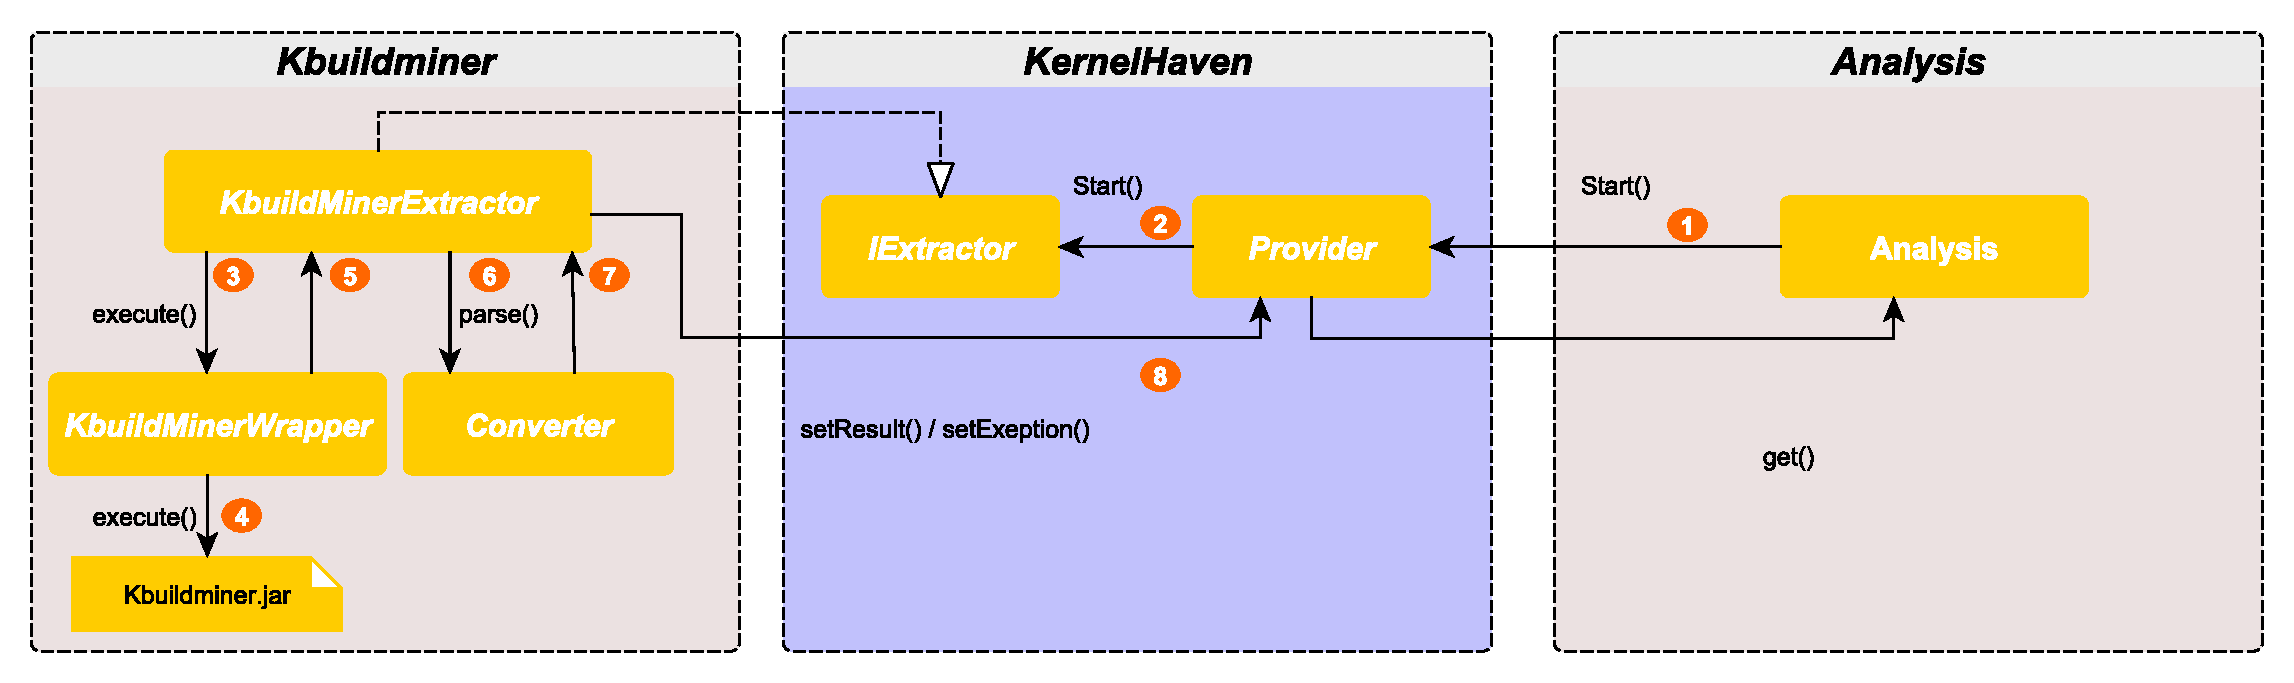
\includegraphics[scale=0.4]{Bilder/Pipeline}
  \caption{The process of the pipeline} \label{fig:pipelineprocess}
\end{figure}


\chapter{Writing a new Extractor}
 
\section{Overview}

An extractor class has to implement the following Methods:
\begin{itemize}
    \item Implement \texttt{IBuildModelExtractor}, \texttt{IVariabilityModellExtractor} or \newline \texttt{ICodeModelExtractor} with the following methods:
    \begin{itemize}
        \item \textbf{\texttt{setProvider()}} is called in the setup phase to tell the extractor which provider it should send its results to.
        \item \textbf{\texttt{start()}} is called by the Provider to signal the extractor that it should start its extraction process. The extraction process should run in a seperate thread.
        \item \textbf{\texttt{stop()}} is called by the Provider to signal that the extraction process took too long and the extractor should abort its extraction process.
    \end{itemize}
\end{itemize}

The extractor has to use one of the following methods to signal the Provider its result. Those methods need to be called directly on the provider instance that was passed via the \texttt{setProvider()} method.:
\begin{itemize}
    \item \textbf{\texttt{setResult()}} can be called to give the extractor the result of the extraction process. This must not be called after the provider called \texttt{stop()} (see above).
    \item \textbf{\texttt{setException()}} can be called instead of \texttt{setResult()}, to tell the Provider that the extraction process has terminated with an exception. The exception passed to it will be thrown in the next \texttt{getResult()} call that the analysis does on the provider.
\end{itemize}

If none of these methods is called within a user configured timeout, then the provider will kill the extractor via the \texttt{stop()} method.

There also needs to be a factory for creating an instance of the extractor for a given configuration. This factory needs to implement \texttt{IBuildExtractorFactory}, \texttt{ICodeExtractorFactory} or \texttt{IVariabilityExtractorFactory}. This interface defines the following method to be implemented:
\begin{itemize}
    \item The \textbf{create()} method gets the configuration for the extractor and should return an instance of it. This is called via reflection when the analysis starts the extraction process. This method may throw a \texttt{SetupException} if it detects any invalid configuration options.
\end{itemize}

\section{Example}

Here is an example implementation of a build model extractor:

\lstinputlisting[language=Java]{DummyBuildExtractor.java}

This extractor has a configuration property that either tells it to return an empty \texttt{BuildModel} or throw an \texttt{ExtracorException}.

The following factory can be used to instantiate this extractor:

\lstinputlisting[language=Java]{DummyBuildExtractorFactory.java}

To compile this in eclipse:
\begin{itemize}
    \item Create a new project
    \item Add the kernelhaven.jar with source attachments to the build path
    \item Insert the two classes from above
    \item Export the project as a jar archive (not as a runnable jar)
\end{itemize}

To run this extractor in the infrastructure, place the jar file in the plugins folder and set the factory at the build model extractor in the properties (see user documentation for details on this).




%################################## Analysis section ###################################################
\chapter{Writing a new Analysis}
\label{sec:Analysis}
\section{Overview}

An analysis class has to implement the following Methods:
\begin{itemize}
    \item Extend the abstract \texttt{AbstractAnalysis} class. The analysis has to implement the following abstract methods of it:
    \begin{itemize}
        \item \textbf{\texttt{run()}} is called by the infrastructre after the pipeline is set up. This should execute the analysis.
    \end{itemize}
    \item A \textbf{constructor}  which takes a \texttt{Configuration} object. This is called via reflection in the setup phase to instantiate the analysis. The configuration object passed to it is the user configuration. This constructor may throw a \texttt{SetupException} if it detects any invalid configuration options.
\end{itemize}
The analysis can use the following API:

\begin{itemize}
    \item The variables \textbf{\texttt{vmProvider}}, \textbf{\texttt{bmProvider}} and \textbf{\texttt{cmProvider}} give it access to the providers. These first need to be started via their \texttt{start()} methods. The configurations required by the \texttt{start()} methods can be derived from the configuration passed to the constructor.
    
    After the start methods have been called, the extractors run asynchronously. The result can be queried via the \texttt{getResult()} methods; this method blocks until the result is ready (or an \texttt{ExtractorException} is thrown).
    \item \textbf{\texttt{createResultStream()}} can be called to create a stream to a file to write the result of the analysis to. The infrastructure takes care that the result file is created in the correct output directory.
    \item The variable \textbf{\texttt{LOGGER}} can be used to log progress, etc.
\end{itemize}

To keep the analysis re-usable by other analyses, it should contain a public method that does the main analysis. The \texttt{run()} method should only start the providers and call this analysis method.

\section{Example}

The following example contains a \texttt{doAnalysis()} and a \texttt{run()} method which may seem redundant initially. However this setup can be beneficial when one analysis uses components of another analysis. While the \texttt{run()} method starts the providers that does not need to be done when called from another analysis as that part has already be taken care of by the calling analysis. Instead the calling analysis may use \texttt{doAnalysis()} and thereby only run the analysis-part without starting any further extractor-processes.

\lstinputlisting[language=Java]{DummyAnalysis.java}

To compile this in eclipse:
\begin{itemize}
    \item Create a new project
    \item Add the kernelhaven.jar with source attachments to the build path
    \item Optional: Add other dependencies (like CnfUtils) to the build path
    \item Insert the analysis class from above
    \item Export the project as a jar archive (not as a runnable jar)
\end{itemize}

To run this analysis in the infrastructure, place the jar file containing the analysis class in the plugins folder. Then set the analysis setting in the properties file to the fully qualified class name of your analysis (see the user documentation for details on this).



% utility Plugins ####################################################################################################

\section{Utility Plugins for Analyses}


CnfUtils is a project distributed with every release of KernelHaven as binary-jar as well as source code. It contains common operators for handling cnf. Refer to the javadoc/sourcecode for detailed information.

CnfUtils-Overview:

\begin{description}
    \item[Cnf] \hfill \\
    Cnf is a storage class for storing boolean formulas in conjunctive normal form.
    \item[SatSolver]\hfill \\
    This class is used to check if an instance of \texttt{Cnf} is satisfiable.
    \item[FormulaToCnfConverterFactory]  \hfill \\
    This factory can create converters which convert a boolean \texttt{Formula}  to \texttt{Cnf}.
    \item[VmToCnfConverter]  \hfill \\
    Converts a variablity model with a constraint model file in \texttt{DIMACS} to a \texttt{Cnf} object.
\end{description}
